\documentclass[../main.tex]{subfiles}

\makeatletter
\@ifundefined{fromRoot}{%
  \newcommand{\fromRoot}[1]{../#1}
  
 % \usepackage{xr}
  % \externaldocument{../main}
}{}

\def\input@path{{\subfix{../}}}
%or: \def\input@path{{/path/to/folder/}{/path/to/other/folder/}}
\makeatother

\graphicspath{
  {\subfix{../}}
  {\subfix{./figures}}
  {\subfix{../figures}}
  {\subfix{./figures/logos-thesis/}}
  {\subfix{../figures/logos-thesis/}}
  {\subfix{./figures/rtexps-pics/}}
  {\subfix{../figures/rtexps-pics/}}
}

\hypersetup{
    pdfauthor   = {Camille MONIÈRE},
    pdftitle    = {Th\`{e}se (Présentation: conclusion)},
    pdfsubject  = {Th\`{e}se (Présentation: conclusion)},
%    pdfkeywords = {mots-cl\'{e}s},
}

\begin{document}

\section{Conclusion et Perpectives}

\subsection{Synthèse}

\begin{frame}{\subsecname}
  \begin{columns}
    \begin{column}{.7 \linewidth}
      \begin{ctrlitemize}{1 em}
        \item L'algorithme préexistant a été amélioré :
        \begin{ctrlitemize}{.5 em}
          \item Robustesse aux variations de gain d'entrée ;%|
          \item Rapport $\frac{\text{performances de détection}}{\text{complexité calculatoire}}$ supérieur ;
          \item Objectif de performances atteint {\tiny (SNRs inférieurs à $-10$ dB, avec $20 \%$ de ressource spectrale de moins comparé aux protocoles à base de préambules \cite{saiedThesis2022})}.
        \end{ctrlitemize}
        \item Le  récepteur QCSP est temps réel ($\approx 100$ kb/s de débit utile), grâce aux efforts de parallélisation ;
        \item Des campagnes d'expérimentations grandeurs nature ont permis, et permettent encore, d'améliorer le modèle et l'algorithme ;
      \end{ctrlitemize}
    \end{column}
    \begin{column}{.3 \linewidth}
      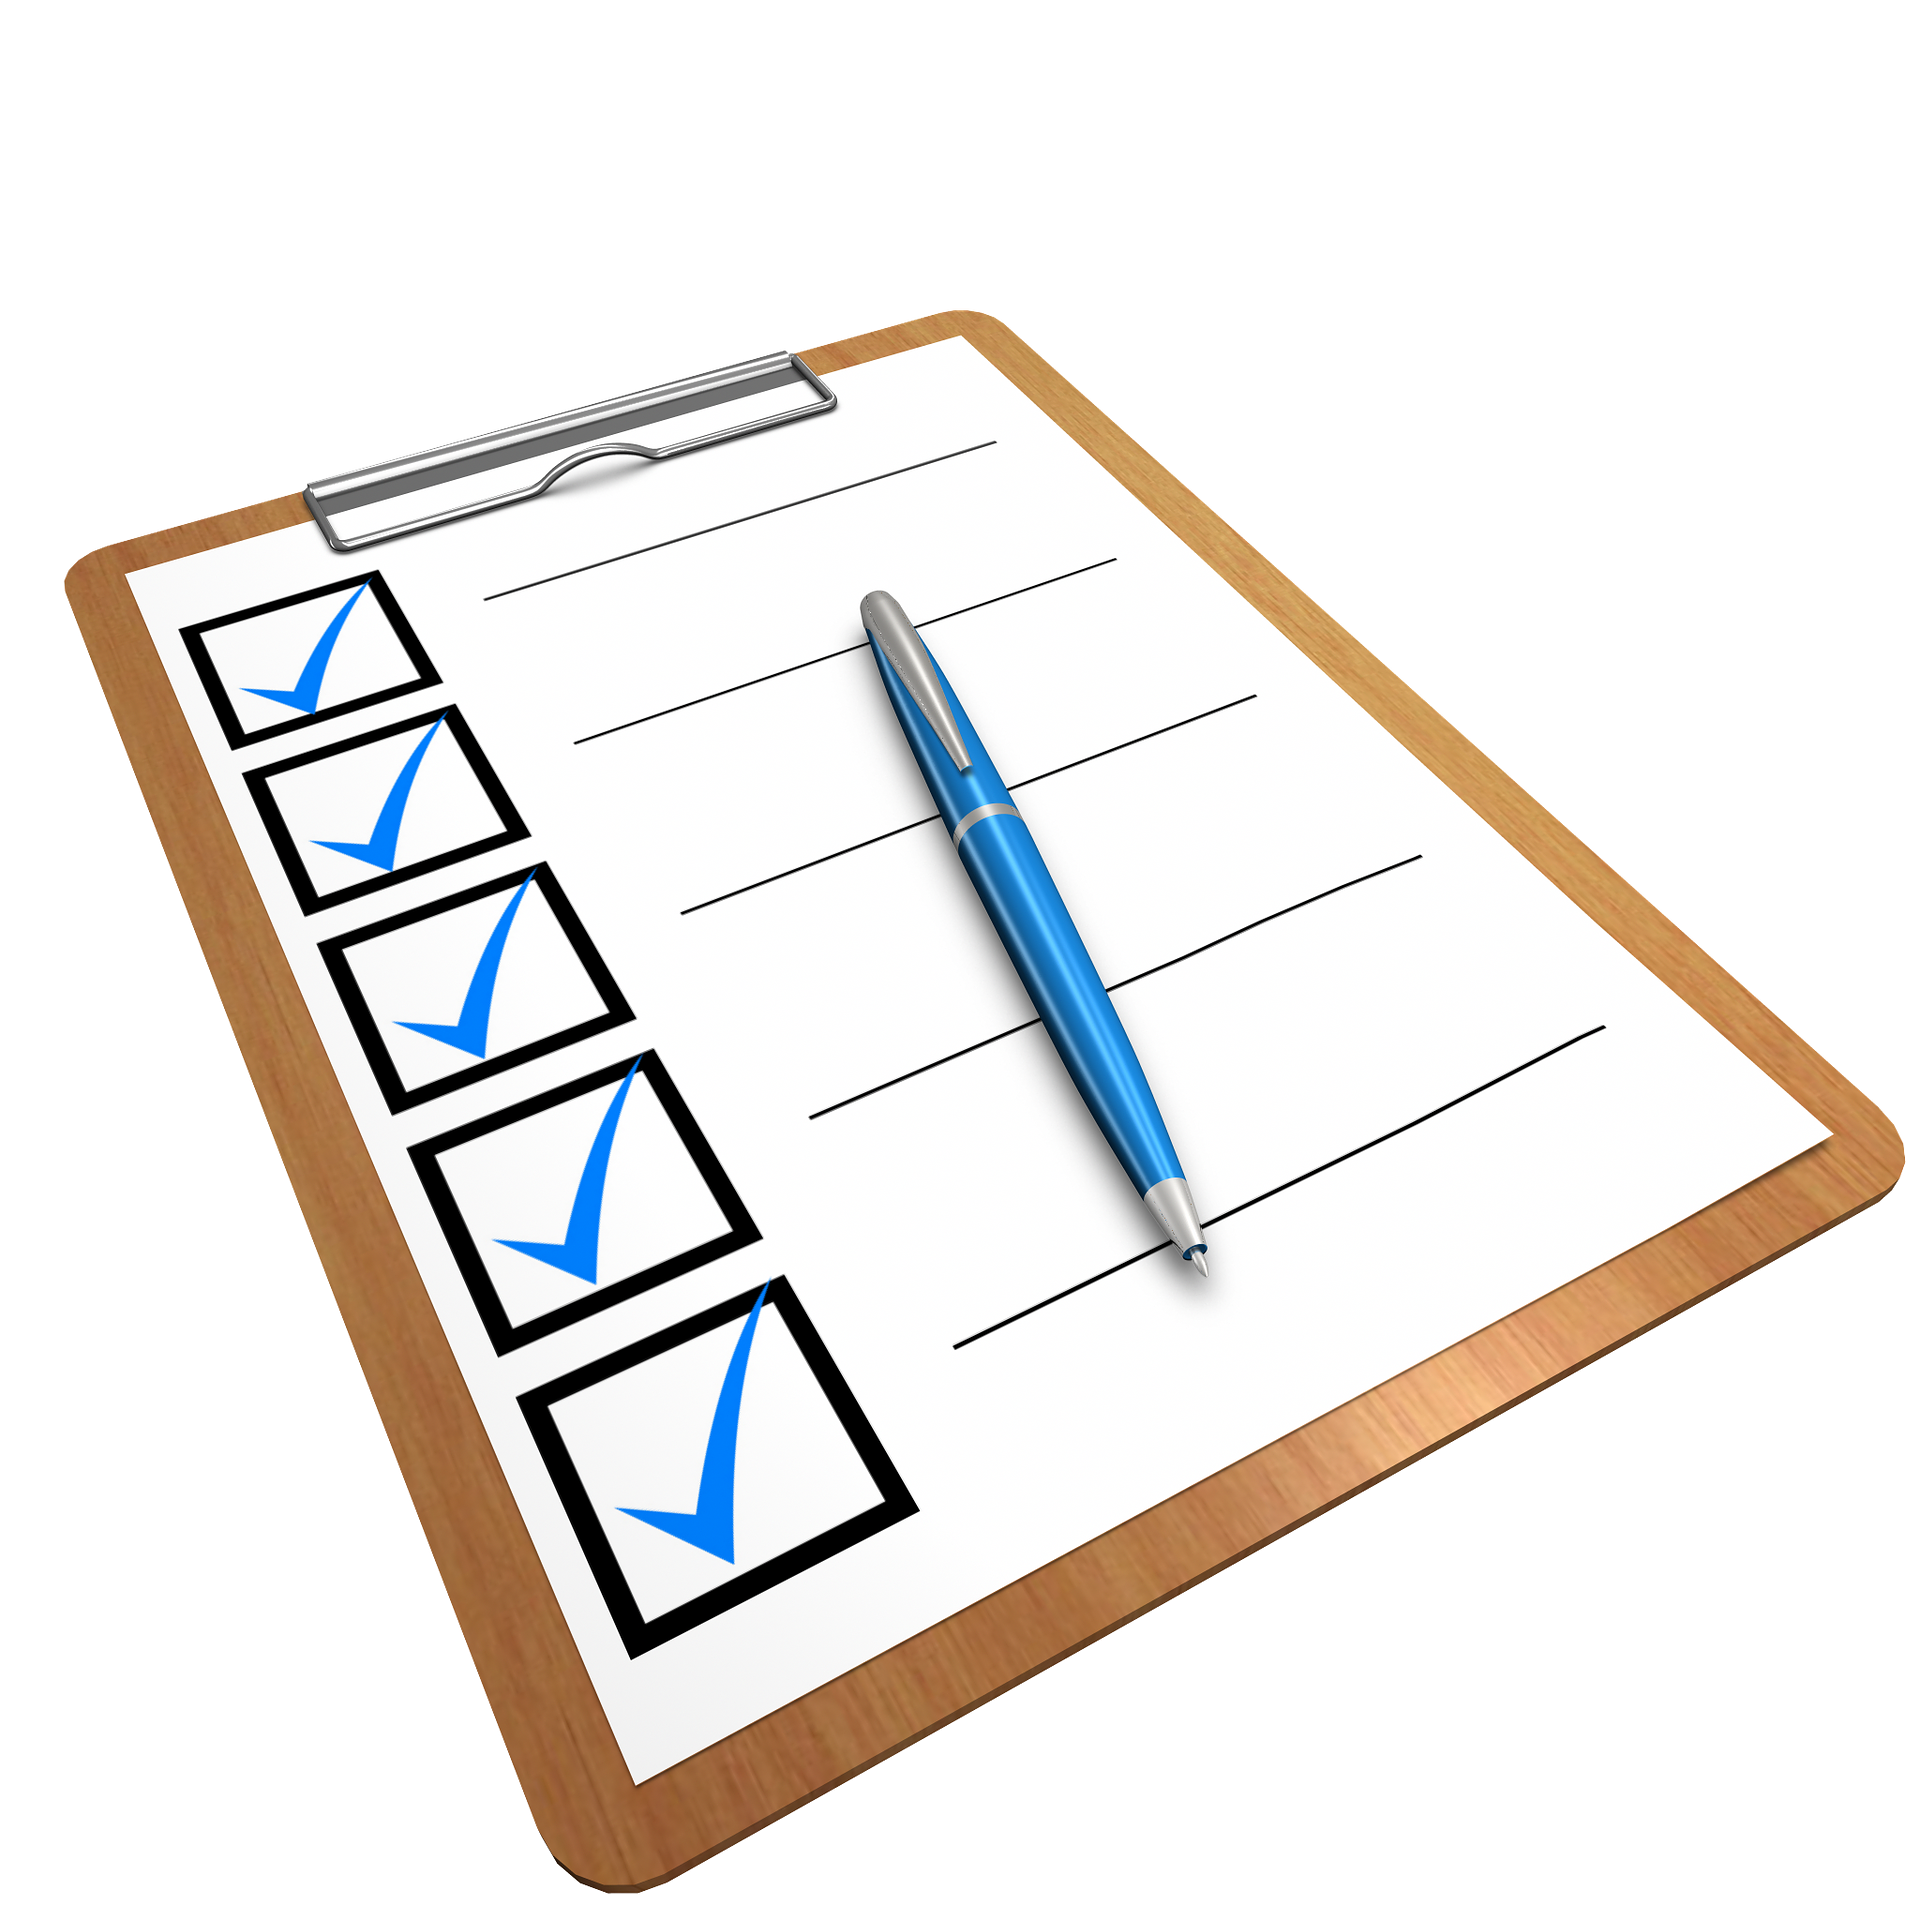
\includegraphics[width = \linewidth]{checklist-1622517_1920.png}
    \end{column}
  \end{columns}
  \blfootnote{\textcite{saiedThesis2022}}
\end{frame}

\subsection{Contributions}
\begin{frame}
  \frametitle{\subsecname}
  \scriptsize
  \begin{refsection}
    \nocite{*}
    Article soumis à une revue internationale

    \vspace{.5 em}

    \renewcommand*{\bibfont}{\rikiki}
    \printbibliography[keyword=ownpub, keyword=inter, type=article, heading=none,]

    \vspace{1 em}

    Papiers en conférences internationales

    \vspace{.5 em}

    \renewcommand*{\bibfont}{\rikiki}
    \printbibliography[keyword=ownpub, keyword=inter, type=inproceedings, heading=none,]

    \vspace{1 em}

    Papiers en conférences nationales

    \vspace{.5 em}

    \renewcommand*{\bibfont}{\rikiki}
    \printbibliography[keyword=ownpub, keyword=nationale, type=inproceedings, heading=none,]
    \printbibliography[keyword=ownpub, keyword=nationale, type=misc, heading=none,]

    \vspace{1 em}
    Intervention dans des colloques nationaux

    \vspace{.5 em}

    \renewcommand*{\bibfont}{\rikiki}
    \printbibliography[keyword=ownpub, keyword=nationale, type=unpublished, heading=none,]

  \end{refsection}
\end{frame}

\subsection{Perspectives futures}

\begin{frame}{\subsecname}
  \begin{columns}
    \begin{column}{.7 \linewidth}
      {\centering \underline{\textbf{Courts termes}}\par}
      \begin{ctrlitemize}{.6 em}
        \item Modèle en virgule fixe validé, en cours d'implantation sur puce FPGA ;
        \item Intégration complète du détecteur FPGA dans un module radio-logiciel.
      \end{ctrlitemize}

      {\centering \underline{\textbf{Longs termes}}\par}
      \begin{ctrlitemize}{.6 em}
        \item Porter les avancées de la détection à la synchronisation ;
        \item Étudier la faisabilité d'un récepteur QCSP sur un SoPC ;
        \item Étudier la modularité de la chaines QCSP --- Différentes complexités potentielles pour différents usages.
      \end{ctrlitemize}
    \end{column}
    \begin{column}{.3 \linewidth}
      \hfill 
\includegraphics[width = .35\linewidth]{future_sp.png} \\
      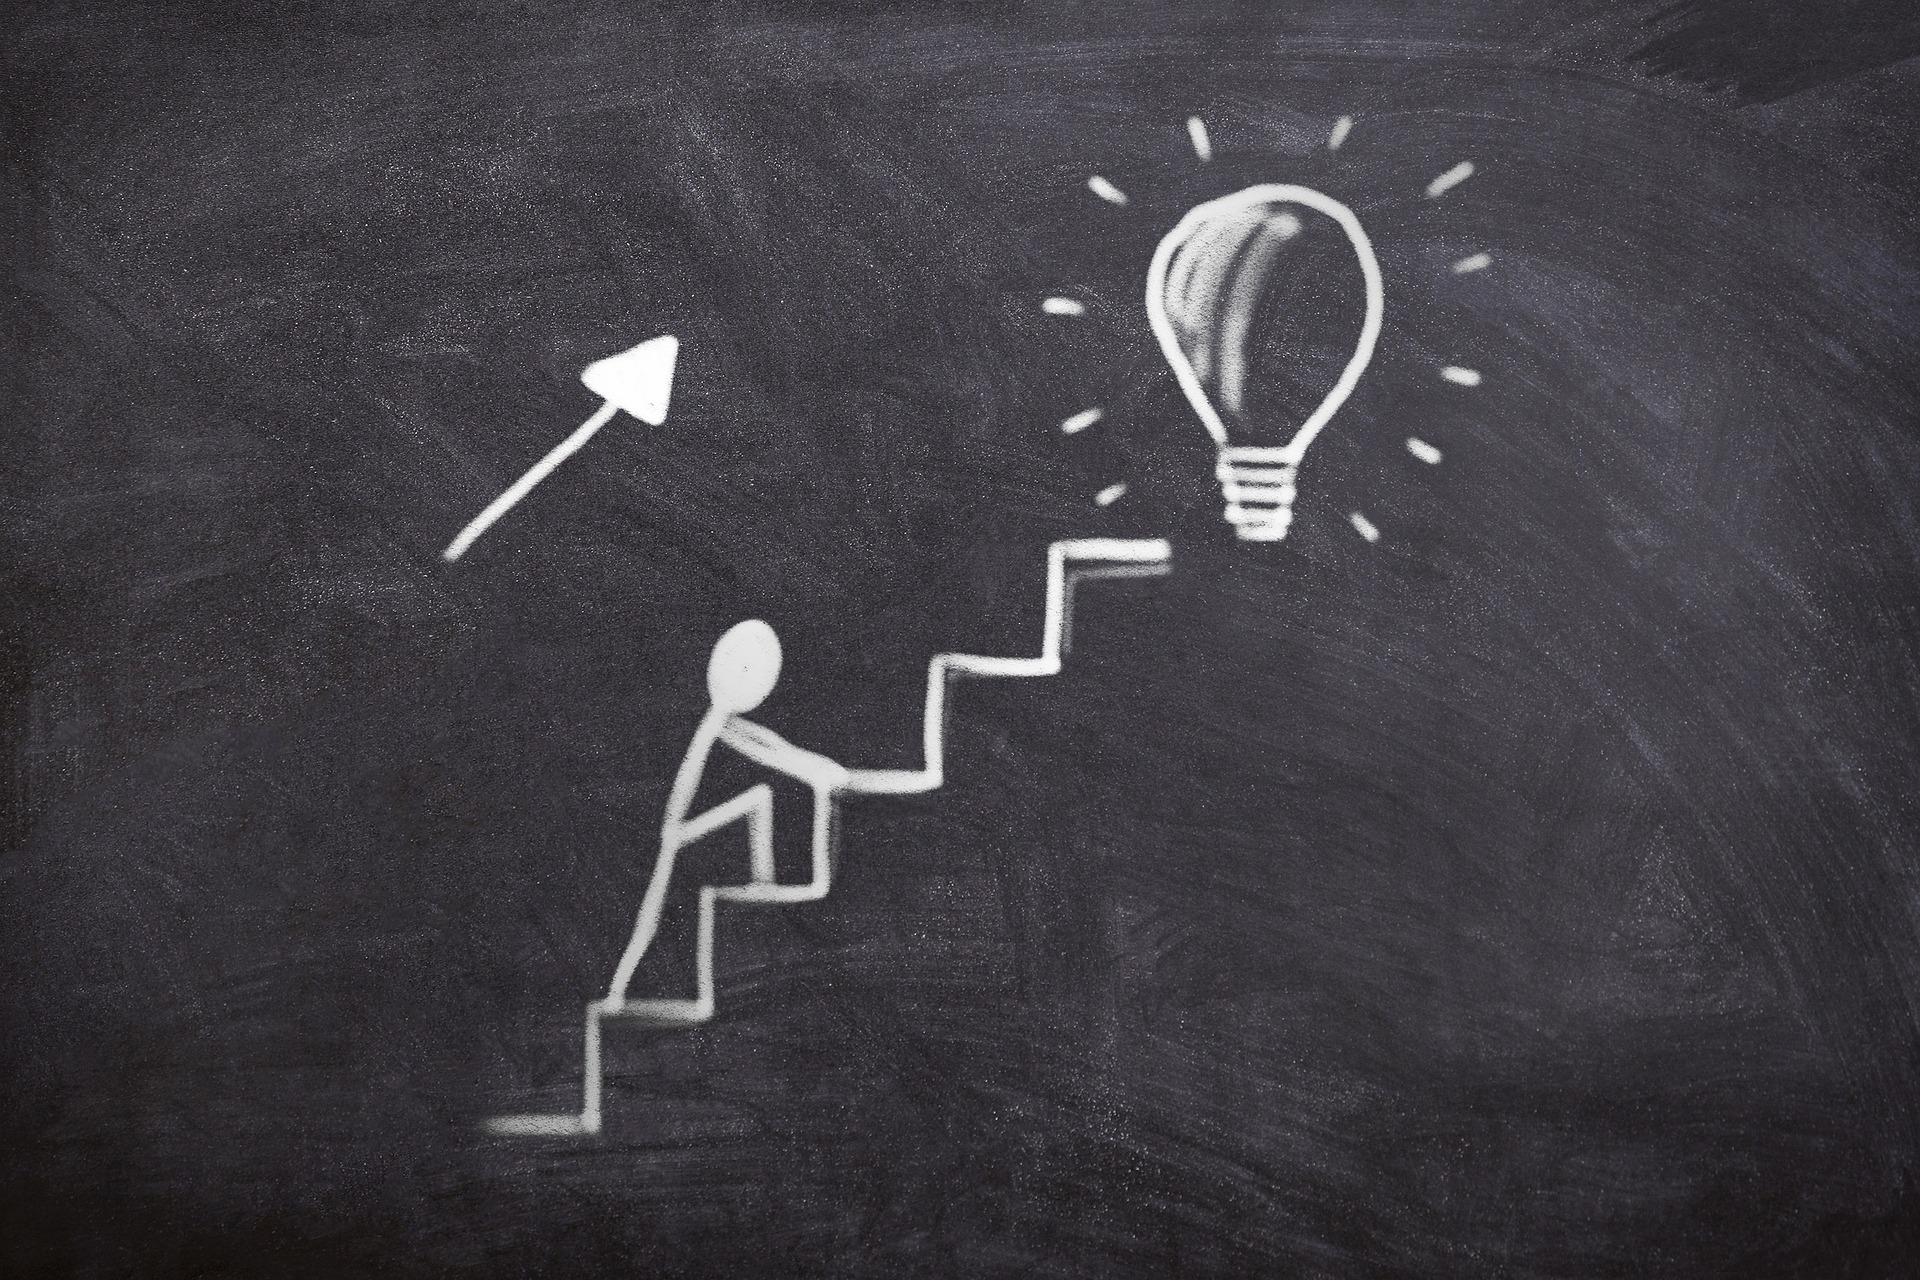
\includegraphics[width = \linewidth]{steps_futur.jpg}
    \end{column}
  \end{columns}
\end{frame}


\end{document}
